\documentclass[a4paper]{article}
\usepackage{calc}
\usepackage{verbatim}
\usepackage{alltt}
\usepackage{graphicx}
\usepackage{url}

\newlength{\myrightmargin}
\newlength{\myleftmargin}
\newlength{\mytopmargin}
\newlength{\mybottommargin}

% Change these settings to change the margins
\setlength{\myrightmargin}{1.0in}
\setlength{\myleftmargin}{1.0in}
\setlength{\mytopmargin}{0.5in}
\setlength{\mybottommargin}{1in}
\setlength{\oddsidemargin}{0.0in}   % extra room on inside side

%%% use margin settings to set width variables
\setlength{\evensidemargin}{0 in}
\setlength{\marginparsep}{0 in}
\setlength{\marginparwidth}{0 in}
\setlength{\hoffset}{\myleftmargin - 1.0in}
%\setlength{\textwidth}{8.5in -\myleftmargin -\myrightmargin -\oddsidemargin}
\setlength{\textwidth}{21cm -\myleftmargin -\myrightmargin -\oddsidemargin}

%%% use margin settings to set height variables
\setlength{\voffset}{\mytopmargin -1.0in}
\setlength{\topmargin}{0 in}
\setlength{\headheight}{12 pt}
\setlength{\headsep}{20 pt}
\setlength{\footskip}{36 pt}
%\setlength{\textheight}{11.0in-\mytopmargin-\mybottommargin-\headheight-\headsep-\footskip}
\setlength{\textheight}{29.8cm-\mytopmargin-\mybottommargin-\headheight-\headsep-\footskip}

\setlength{\parindent}{0cm}
\setlength{\parskip}{.5ex}

\newenvironment{source}%
% begin environment
{\begin{alltt}\footnotesize}%
% end environment
{\end{alltt}}

\input{version}

\begin{document}

\title{ADP Compiler \rsversion{} manual}

\author{Peter Steffen$^{\rm 1}$, Marco R\"uther, Christian Lang\\ 
    and Georg Sauthoff\\[.5cm] 
    $^{\rm 1}$Faculty of Technology, Bielefeld University, 33594
    Bielefeld, Germany, \\
    email: psteffen@techfak.uni-bielefeld.de}

\maketitle
\tableofcontents

\section{Introduction}

This manual gives a short overview of the ADP
compiler. Section~\ref{sec:start} gives an exemplified introduction
to the ADP compiler's compilation process. Section~\ref{sec:options}
then gives a complete account of the compiler's command line interface.

This manual does not contain any information about the internals of
the ADP compiler. See Peter Steffen's PhD thesis (file
\texttt{diss.pdf} in the compiler distribution) for some internal
details of the ADP compiler.

\section{Quickstart}
\label{sec:start}

Copy the file \texttt{ElMamun.lhs} out of the directory
\texttt{INSTALLDIR/share/adpc/examples}. Then type 

\texttt{adpc ElMamun.lhs}

This generates a number of files, the most important ones the files
\texttt{Makefile} and \texttt{ElMamun.xml}. The file \texttt{Makefile}
contains the compile targets necessary to compile \texttt{ElMamun.lhs}
into the desired C target code files. In the next step, simply type

\texttt{make}

This generates the main target file \texttt{ElMamun.c} and for every
algebra in the source file (\texttt{seller}, \texttt{buyer},
\texttt{count}) a target code file \texttt{ElMamun\_{\it algebra}.c}.
These target files are then each compiled by the C compiler
\texttt{gcc} and linked together to the executable binary file
\texttt{ElMamun}. See Figure~\ref{fig:adpc} for an overview of the
compilation process.

\begin{figure}[htbp]
  \centering
  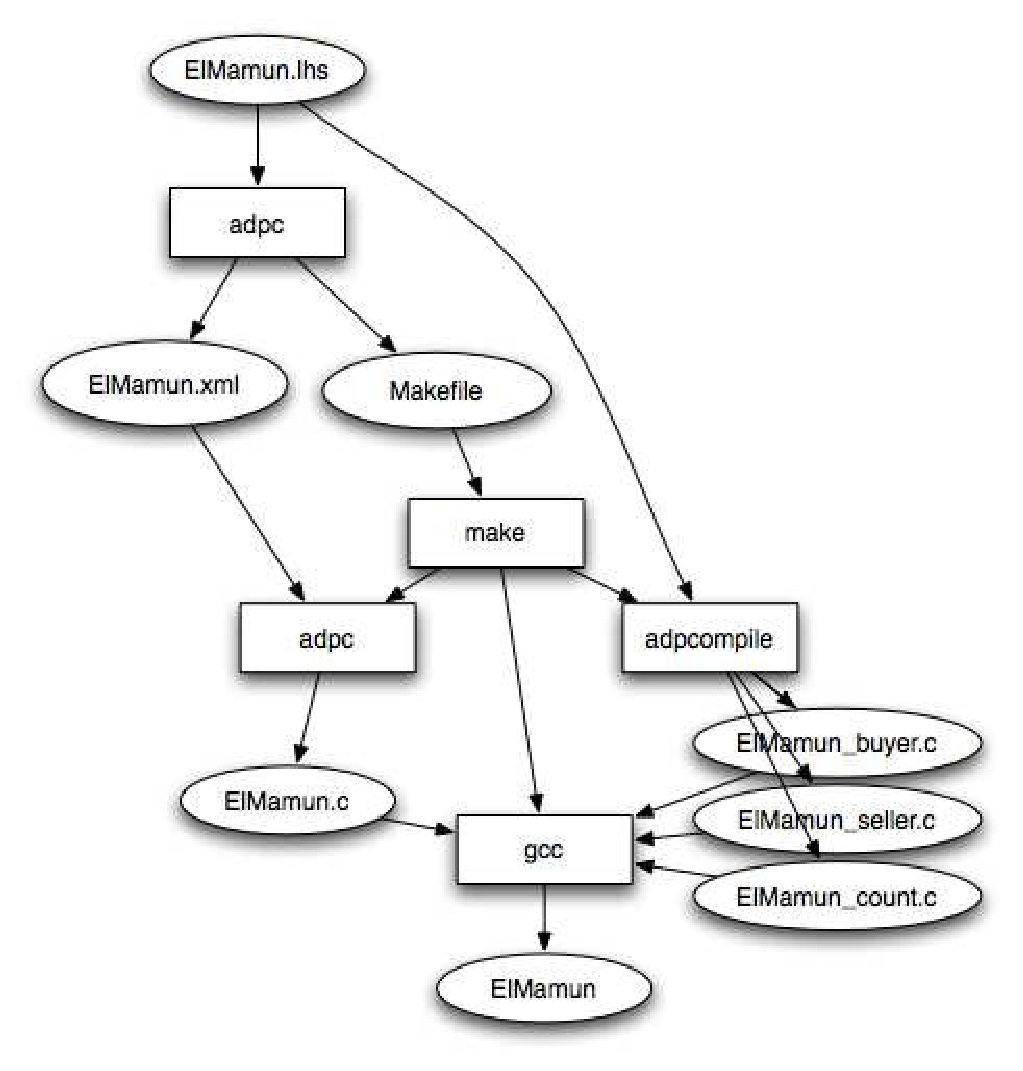
\includegraphics[width=\linewidth]{adpc-framework.pdf}
  \caption{Adpc framework}
  \label{fig:adpc}
\end{figure}

After the compilation finished, you can simply start \texttt{ElMamun}
by typing

\texttt{./ElMamun}

This gives the following interactive command line:

\begin{verbatim}
Welcome to ElMamun!

ElMamun> 
\end{verbatim}

At the command prompt you need to type a formula that shall be
evaluated by the ElMamun program. For example, type:

\texttt{ElMamun> 1+2*3*4+5}

This gives the following result:

\begin{verbatim}
ElMamun> 1+2*3*4+5

Input: 1+2*3*4+5
Algebra: count, score: 51

=================================================================

Input: 1+2*3*4+5
Algebra: buyer, score: 30
Suboptimal range: [30 - 35]

 Score | Candidate
-----------------------------------------------------------------
    30 | ((1+((2*3)*4))+5)
    30 | ((1+(2*(3*4)))+5)
    33 | (((1+(2*3))*4)+5)
    30 | (1+(((2*3)*4)+5))
    30 | (1+((2*(3*4))+5))
    35 | (1+(2*((3*4)+5)))

=================================================================

Input: 1+2*3*4+5
Algebra: seller, score: 81
Suboptimal range: [76 - 81]

 Score | Candidate
-----------------------------------------------------------------
    81 | (((1+2)*3)*(4+5))
    81 | ((1+2)*(3*(4+5)))

=================================================================
ElMamun> 
\end{verbatim}

The first result shown is the result for algebra \texttt{count}. It
states that there are 51 ways to evaluate the formula. The second
result is the result for algebra \texttt{buyer}. It is a minimizing
algebra, and the best score for the formula is 30. The list below
shows six results that occur in the suboptimal range of 30 to 35. The
last result then shows the results for algebra seller. It is a
maximising algebra, and the best score for this input is 81. There
exist two candidates that achieve this score.

Repeat this compilation process with the second program in the
examples directory, \texttt{RNAfold.lhs}.

\section{The ADP compiler's command line interface}
\label{sec:options}

The ADP compiler consists of two executable programs. The program
\texttt{adpc} is responsible for creating the main program interface
of the target program, the \texttt{Makefile}, and several other parts.
Apart from the name of the input file, \texttt{adpc} has no command
line options.  The \texttt{Makefile} then contains the calls to the
main ADP compiler executable, \texttt{adpcompile}. This program does
the main work of the ADP compiler and has a lot of command line
options. See the \texttt{Makefile} for a typical command line call.
In a typical application setting, you do not need to call
\texttt{adpcompile} directly. This is done automatically by the
\texttt{Makefile}. But there exist cases where it is necessary to call
\texttt{adpcompile} separately from the \texttt{adpc} program flow. In
these cases, you need to take care of the \texttt{adpcompile} command
line options.  The following section gives a complete description of
the \texttt{adpcompile} command line interface.

\input{options}

\end{document}
